\chapter{Methods}
\label{ch:methods}

\section{Method}
\label{sec:main}
Our objective is to evaluate the capacity of existing LiDAR place recognition models to successfully produce robust loop closure candidates within dense forest environments. Our evaluation considers three distinct tasks: 
\begin{itemize}
  \listparindent=-20pt
  % \itemindent=-10pt
  \item \emph{Task A: Online SLAM}: the proposed loop candidates contributing to a globally-consistent pose graph mapping system in an incremental manner.
  \item \emph{Task B: Offline multi-mission SLAM}: loop candidates used to link different physically overlapping missions collected at different times.
  \item \emph{Task C: Relocalization}: place recognition in a prior map made up of individual scans enabling autonomy within the map such as longer term monitoring or harvesting.
\end{itemize}

Our system infrastructure is shown in \figref{fig:pipeline}. For state estimation, we use a LiDAR-inertial odometry system---VILENS~\cite{wisth2023tro}---, in conjunction with a pose graph SLAM framework~\cite{proudman2022ras}. Additionally, we implemented a \emph{place recognition \& verification server}, which not only provides a common interface for the different LiDAR-based place recognition models but also multi-stage verification procedures for its use in the different proposed tasks.

In the following sections, we present the technical details of the place recognition server, and then we present its integration to solve the three aforementioned tasks.

%\mfallon{The Wisth paper is an odometry system - not the SLAM system. We have no SLAM system paper. You can refer to Proudman's paper
%`As a basis we use the VILENS lidar-inertial odometry system and a pose graph SLAM. See Proudman et al where this is described in more detail'}
%\mfallon{Please make Fig 2 show "VILENS Lidar Inertial Odometry" and Pose Graph SLAM (without VILENS)}
%\haedam{Edit figure and text accordingly}

% \mfallon{Above you say `we too VILENS and merged it with Logg3dNet. But we want to present the paper as a study of the different methods followed by further experiments with Logg3dNet. So remove the reference above.}

% \haedam{changed last sentence pretending we integrated all four models. Nived can you check this?}
% \mfallon{you are missing the formalism which says that `the prior map is made up a set of V nodes each with a point cloud and a representative pose'. You need not say `pose graph' because the only difference between Online SLAM and relocalisation is the nodes positions is that the list of nodes continuously.}
% \haedam{Haedam: I added Joe's figure, and will explain this more clearly in next section}

\begin{figure}[t]
  \centering
  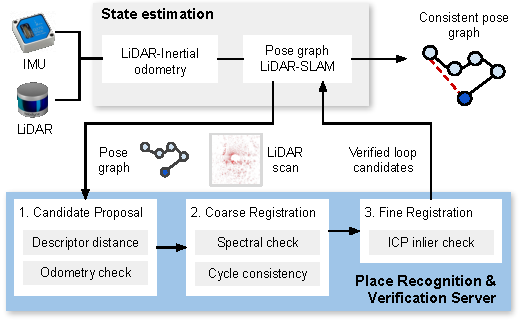
\includegraphics[width=\columnwidth]{pics/method_pipeline.pdf}
  \caption{Our place recognition pipeline. VILENS provides a continuous odometry estimate at 10 Hz. Pose graph SLAM is used to optimize poses after successful loop closure verification. 
  The place recognition module consists of three steps: Loop candidate proposal, coarse registration, and fine registration. We verify loop candidates
  at the global descriptor-level, local feature-level consistency, and finally fine registration level. A loop candidate is integrated in the pose graph only if it passes these three stages.}
  \label{fig:pipeline}
\end{figure}


% Overall Pipeline
% This star removes this subsection from the A,B,C list. Such that the task A,B,C match
\subsection*{Place Recognition \& Verification Server} \label{sec:pipeline}\haedam{reference to method figure which step is which}
Our place recognition pipeline consists of three steps: loop candidate proposal, coarse registration, and a final fine-registration. At each step, we perform appropriate checks to filter out incorrect loop closures.

The main inputs are the pose graph, with corresponding LiDAR scans attached to each pose, as well as the single query scan. The query scan is provided by different sources depending on the task we are solving. For example, in the relocalization task it will be a live scan directly from the LiDAR sensor. Further details are provided in the corresponding sections.

% 1.1 Descriptors (Descriptor distance,)
\subsubsection{\textbf{Step 1: Loop candidate proposals}}
\label{subsubsec:loop-candidate}
Initial loop closure candidates are obtained by comparing global descriptors extracted from the pose graph scans as well as the query scan. In this paper, we evaluate four state-of-the-art methods for descriptor extraction: the learning-based Logg3dNet~\cite{vidanapathirana2022icra} and EgoNN~\cite{komorowski2022ral}, as well as the handcrafted ScanContext~\cite{kim2018iros} and STD~\cite{yuan2023icra}.

Given the reference pose graph and the query scan, we compute a database of descriptors using all the scans in the pose graph, given by the matrix $\mathbf{D} \in \R{N\times M}$, where $N$ is the number of poses in the pose graph and $M$ the descriptor dimension. Additionally, we compute the descriptor for the query scan, denoted by $\mathbf{d}_{q} \in \R{M \times 1}$. 

To obtain candidates, we simply compute the pairwise distances of the scan to the database using the cosine similarity:
\begin{equation}
  \mathbf{S} = \mathbf{D} \cdot \mathbf{d}_{q} \in \R{N \times 1}
\end{equation}
The vector of descriptor distances $\mathbf{S}$ is sorted by increasing distance, and only the top-$k$ candidates are selecting using a distance threshold $\tau_{s}$.

\mfallon{we should discuss this comment here - I dont know what it means:}
If a spatial prior is available, for example from LiDAR-inertial odometry, we also perform an additional spatial check discarding all the candidates that are more than \SI{20}{\meter} away from the query scan. The output is a set of candidate nodes $\{ n_c\}$.

% 2.1 Pose Estimation (RANSAC) ... notation is a bit confusing.
\subsubsection{\textbf{Step 2: Coarse Registration}}
\label{subsubsec:coarse-registration}
Next, we estimate the relative 6DoF transformation that expresses the pose associated to the query scan w.r.t each candidate node, which we denote $\Delta \mathbf{T}$. For the handcrafted methods (ScanContext and STD), the relative transformation is directly an output of descriptor computation. For the learning-based approaches, we use the point-wise feature vectors outputted in the forward pass of Logg3dNet and EgoNN for point matching, which is used in a RANSAC-based pose estimation scheme~\cite{fischler1981ransac} to obtain the estimated relative transformation.

% \mfallon{please search for `relative' thoughout the paper and check that you use `relative transformation' not `relative pose'.}

% 2.2 SGV
We additionally verify the inlier matches using the \emph{Spectral Geometric Verification}~\cite{vidanapathirana2023ral} method, which provides an additional measure of the quality of the feature matches.

Lastly, we carry out a \emph{cycle consistency} verification, which checks whether the relative transformations between pairs of nodes are mutually consistent with one another. In brief, when given four pose graph nodes $n_i, n_j, n_k, n_l$, we test how close the following equivalence holds:
\begin{equation}
\Delta\mathbf{T}_{i,j}\, \Delta\mathbf{T}_{j,k}\, \Delta\mathbf{T}_{k,l}\, \Delta\mathbf{T}_{l,i}\, \approx \mathbf{I}_{4\times4} 
\end{equation}
If the difference around a cycle is more than a threshold of \SI{10}{\centi\meter} and \SI{1}{\degrees} we reject the candidate. This is shown in \figref{fig:cycle-consistency}, please refer to the corresponding sections for further details.

The interpretation of these transformations change if we discussing online SLAM (\secref{sec:online_slam_mode}), offline multi-mission SLAM (\secref{sec:offline}), or pure relocalization (\secref{sec:relocalization}). 

\begin{figure}[t]
  \centering
  \includegraphics*[width=\columnwidth]{pics/methods_pairwise_consistency.pdf}
  \caption{Our proposed cycle consistency check is general and applies to the online and offline multi-mission SLAM case, as well as relocalization tasks. We only need the relative transformation estimates and loop candidates between four nodes $n_i, n_j, n_k, n_l$ to verify the validity of a loop. Please refer to \secref{subsubsec:coarse-registration} for technical details.}
  \label{fig:cycle-consistency}
\end{figure}

% 3. ICP 
\subsubsection{\textbf{Step 3: Fine Registration}}
\label{subsubsec:fine-registration}
Finally, we employ the Iterative Closest Point (ICP) algorithm~\cite{besl1992icp} for fine registration of the proposed candidates. We use the \emph{libpointmatcher} implementation~\cite{pomerleau2013iros}, which also provides information on the quality of the registration, such as the proportion inlier points and the Residual Error of each point to access the alignment.
% \mfallon{LibPM returns the residual error of each point. My code uses a threshold (20cm) to determine if a point is an inlier. This magic number is really undertuned}
% this magic number of 20cm is very very important:
% https://github.com/ori-drs/vilens/blob/develop/icp_odometry/icp_odometry/src/icp_odometry/registration_verification.cpp#L28

% since the number of points is fixed (20k I think), the number is really a proportion
We use the proportion of inliers and the residual error of \SI{20}{\centi\meter} as a final verification step to reject loop candidates. The verified candidates are then used for SLAM or relocalization tasks, which are detailed in the following sections.

\subsection*{Task A: Online Single-mission SLAM} 
\label{sec:online_slam_mode}
\begin{figure}[t]
  \centering
  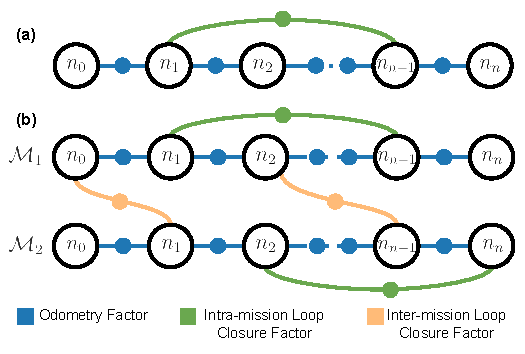
\includegraphics[width=0.99\columnwidth]{pics/factor_graph_v2}
  \caption{Pose graph formulation used for (a) online, and (b) offline multi-mission SLAM optimization. Each node $n_{i}$ has a 6DOF pose $\mathbf{x}_{i}$, which correspond to the main variables estimated on each case.}
  \label{fig:factor_graph}
\end{figure}

The first task we consider is LiDAR-based online SLAM. Our implementation defines it as an incremental pose graph estimation problem (see \figref{fig:factor_graph},(a)). Consider consecutive loop closures at nodes $n_{i}$, $n_{i+1}$ and $n_{j}$, $n_{j+1}$. Edges are provided by relative estimates from our LiDAR-inertial odometry system (odometry factors, denoted by $\Delta\mathbf{T}_{i,i+1}, \Delta\mathbf{T}_{j, j+1}$), and verified loop closure candidates from our place recognition server (loop closure factors, $\Delta\mathbf{T}_{i+1, j}, \Delta\mathbf{T}_{i, j+1}$).
\mfallon{a pose graph is a type of factor graph. no need to say factor graph here}

For the cycle consistency verification described in \secref{subsubsec:coarse-registration}, we consider the relative transformation change between consecutive loop closure candidates w.r.t the pose graph poses and the odometry change (\figref{fig:cycle-consistency}  $i$, $j$, $k$, $l$, replaced by ${i}$, ${i+1}$, ${j}$, ${j+1}$). Again, a cycle consistency needs to be satisfied:
\begin{equation}
  \label{eq:cycle-online}
  \Delta\mathbf{T}_{i,i+1}\, \Delta\mathbf{T}_{i+1, j}\, \Delta\mathbf{T}_{j, j+1}\, \Delta\mathbf{T}_{i, j+1}^{-1} \approx \mathbf{I}_{4\times4}
\end{equation}
\haedam{exp:cycle consistncy works well in this scenario,}
\subsection*{Task B: Offline Multi-Mission SLAM}\label{sec:offline}
Offline multi-mission SLAM addresses the challenge of merging multiple pose graph SLAM missions ${\mathcal{M}_{1, \ldots, n}}$, collected over time, with partly overlapping area. 
The goal is to find inter-mission loop candidates to construct a unified map in a common reference frame. This application is relevant for forestry applications, where it is required to map larger areas by integrating surveys conducted over multiple missions or campaigns.

Unlike the scenario of on-road navigation, where similar routes (hence locations) are revisited, we considered off-road scenarios where the missions are collected in dense forests, where it is often unfeasible to retrace the same paths on each sequence. To avoid inefficiently retracing our steps, we wish to identify loop candidates when passing no closer than about \SI{10}{\meter}, providing the flexibility needed to merge two roughly overlapping missions.

Each mission ${\mathcal{M}_{i}}$ is defined by a pose graph with odometry factors and intra-mission loop closures, obtained during each independent online SLAM run. We aim to provide additional \emph{inter-mission} loop candidates that bridge nodes across missions, as shown in \figref{fig:factor_graph} (b). In this case, loop candidates are obtained by incrementally matching each mission of the nodes on matched missions and corresponding LiDAR scans across the missions.
\mfallon{do you actually do all-v-all? I incrementally build the database graph so its 1v1 and then 2v2.}
\haedam{you're right, we incrementally build it }
For the loop proposal step, we executed the same procedures described in \secref{subsubsec:loop-candidate}, but with the stringent descriptor distance threshold $\tau_{s}$. We observed that in the multi-session case, this was required to allow a larger set of candidates that were later verified by stronger procedures such as the cycle consistency check. 
For the cycle consistency step, we considered pairs of nodes within the same mission, namely $n_i, n_j \in \mathcal{M}_1$ and $n_k, n_l \in \mathcal{M}_2$. The intra-mission relative transformation were then $\Delta\mathbf{T}_{i,j}, \Delta\mathbf{T}_{k, l}$, while the inter-mission relative transformations between loop candidates were given by $\Delta\mathbf{T}_{i,k}, \Delta\mathbf{T}_{j,l}$:
\begin{equation}
  \label{eq:cycle-offline}
  \Delta\mathbf{T}_{i,j}\, \Delta\mathbf{T}_{j,l}\, \Delta\mathbf{T}_{k, l}^{-1}\, \Delta\mathbf{T}_{i,k}^{-1}\, \approx \mathbf{I}_{4\times4}
\end{equation}

\subsection*{Task C: Relocalization} \label{sec:relocalization}
Lastly, we considered the case in which a prior map of the forest was available (from online SLAM). Our place recognition \& verification server could then be used as a relocalization module, by using the loop candidate proposals to produce initial pose estimates, then coarese-to-fine registration achieving real-time localization of the LiDAR sensor base $\B$ with the prior map's coordinate frame $\M$, denoted by $\mathbf{T}_{\M\B}$.

\mfallon{the following paragraph is confusing and poorly written. If we are doing cycle consistency checking we don't have a `successful relocalization' we only have a `possible candidate'}
\mfallon{can you try again?}
\haedam{Okay, I add a sentence above and below}
Similarly to the previous tasks, the main difference is in defining the cycle consistency check. For this case, it is between the current and the last successful relocalization: Given the last relocalization estimate $\mathbf{T}_{\M\B}(t-1)$ and the current estimate $\mathbf{T}_{\M\B}(t)$, we compared the  against the odometry estimates at the same timestamps $\mathbf{T}_{\Odo\B}(t-1)$ and $\mathbf{T}_{\Odo\B}(t)$, where $\Odo$ indicates the fixed odometry frame. The cycle consistency check is then defined as:

\begin{equation}
  \label{eq:cycle-relocalization}
  \underbrace{\mathbf{T}_{\M\B}(t)^{-1}\, \mathbf{T}_{\M\B}(t-1)}_{\Delta\mathbf{T} \text{ in $\M$ frame}}  \, \underbrace{ \mathbf{T}_{\Odo\B}(t-1)^{-1}\,  \mathbf{T}_{\Odo\B}(t)}_{\Delta\mathbf{T} \text{ in $\Odo$ frame}} \approx \mathbf{I}_{4\times4}
\end{equation}
This check is used to verify the relocalization estimate, and if successful, ICP is used to fine-localize the LiDAR sensor within the prior map.
\mfallon{again, we need to point out that localisation into a giant point cloud map would be very inconvenient.}

This relocalization capability facilitates various applications, such a enabling a harvester robot to operate autonomously within a prior map or enabling foresters to visualize a rendering of the virtual forest along with important information on a screen in real-time. An example demonstrating this capability is later presented in \secref{sec:exp_relocalization}, where a prior map of the forest is generated using a backpack-based LiDAR mapping system, and a legged robot continuously relocalizes itself within that prior map as part of an inspection task.
\mfallon{please don't over claim - we didnt do this. soften your comments here please}

\mfallon{But Matias: it would be awesome to do what is described here!}
\haedam{I will try this experiment and see if it works.}
